\documentclass[]{article}
\usepackage{lmodern}
\usepackage{amssymb,amsmath}
\usepackage{ifxetex,ifluatex}
\usepackage{fixltx2e} % provides \textsubscript
\ifnum 0\ifxetex 1\fi\ifluatex 1\fi=0 % if pdftex
  \usepackage[T1]{fontenc}
  \usepackage[utf8]{inputenc}
\else % if luatex or xelatex
  \ifxetex
    \usepackage{mathspec}
  \else
    \usepackage{fontspec}
  \fi
  \defaultfontfeatures{Ligatures=TeX,Scale=MatchLowercase}
\fi
% use upquote if available, for straight quotes in verbatim environments
\IfFileExists{upquote.sty}{\usepackage{upquote}}{}
% use microtype if available
\IfFileExists{microtype.sty}{%
\usepackage{microtype}
\UseMicrotypeSet[protrusion]{basicmath} % disable protrusion for tt fonts
}{}
\usepackage[margin=1in]{geometry}
\usepackage{hyperref}
\hypersetup{unicode=true,
            pdftitle={Globalization and Climate Change: Food Trade},
            pdfauthor={Krista Waugh and Andrew Lind},
            pdfborder={0 0 0},
            breaklinks=true}
\urlstyle{same}  % don't use monospace font for urls
\usepackage{color}
\usepackage{fancyvrb}
\newcommand{\VerbBar}{|}
\newcommand{\VERB}{\Verb[commandchars=\\\{\}]}
\DefineVerbatimEnvironment{Highlighting}{Verbatim}{commandchars=\\\{\}}
% Add ',fontsize=\small' for more characters per line
\usepackage{framed}
\definecolor{shadecolor}{RGB}{248,248,248}
\newenvironment{Shaded}{\begin{snugshade}}{\end{snugshade}}
\newcommand{\KeywordTok}[1]{\textcolor[rgb]{0.13,0.29,0.53}{\textbf{#1}}}
\newcommand{\DataTypeTok}[1]{\textcolor[rgb]{0.13,0.29,0.53}{#1}}
\newcommand{\DecValTok}[1]{\textcolor[rgb]{0.00,0.00,0.81}{#1}}
\newcommand{\BaseNTok}[1]{\textcolor[rgb]{0.00,0.00,0.81}{#1}}
\newcommand{\FloatTok}[1]{\textcolor[rgb]{0.00,0.00,0.81}{#1}}
\newcommand{\ConstantTok}[1]{\textcolor[rgb]{0.00,0.00,0.00}{#1}}
\newcommand{\CharTok}[1]{\textcolor[rgb]{0.31,0.60,0.02}{#1}}
\newcommand{\SpecialCharTok}[1]{\textcolor[rgb]{0.00,0.00,0.00}{#1}}
\newcommand{\StringTok}[1]{\textcolor[rgb]{0.31,0.60,0.02}{#1}}
\newcommand{\VerbatimStringTok}[1]{\textcolor[rgb]{0.31,0.60,0.02}{#1}}
\newcommand{\SpecialStringTok}[1]{\textcolor[rgb]{0.31,0.60,0.02}{#1}}
\newcommand{\ImportTok}[1]{#1}
\newcommand{\CommentTok}[1]{\textcolor[rgb]{0.56,0.35,0.01}{\textit{#1}}}
\newcommand{\DocumentationTok}[1]{\textcolor[rgb]{0.56,0.35,0.01}{\textbf{\textit{#1}}}}
\newcommand{\AnnotationTok}[1]{\textcolor[rgb]{0.56,0.35,0.01}{\textbf{\textit{#1}}}}
\newcommand{\CommentVarTok}[1]{\textcolor[rgb]{0.56,0.35,0.01}{\textbf{\textit{#1}}}}
\newcommand{\OtherTok}[1]{\textcolor[rgb]{0.56,0.35,0.01}{#1}}
\newcommand{\FunctionTok}[1]{\textcolor[rgb]{0.00,0.00,0.00}{#1}}
\newcommand{\VariableTok}[1]{\textcolor[rgb]{0.00,0.00,0.00}{#1}}
\newcommand{\ControlFlowTok}[1]{\textcolor[rgb]{0.13,0.29,0.53}{\textbf{#1}}}
\newcommand{\OperatorTok}[1]{\textcolor[rgb]{0.81,0.36,0.00}{\textbf{#1}}}
\newcommand{\BuiltInTok}[1]{#1}
\newcommand{\ExtensionTok}[1]{#1}
\newcommand{\PreprocessorTok}[1]{\textcolor[rgb]{0.56,0.35,0.01}{\textit{#1}}}
\newcommand{\AttributeTok}[1]{\textcolor[rgb]{0.77,0.63,0.00}{#1}}
\newcommand{\RegionMarkerTok}[1]{#1}
\newcommand{\InformationTok}[1]{\textcolor[rgb]{0.56,0.35,0.01}{\textbf{\textit{#1}}}}
\newcommand{\WarningTok}[1]{\textcolor[rgb]{0.56,0.35,0.01}{\textbf{\textit{#1}}}}
\newcommand{\AlertTok}[1]{\textcolor[rgb]{0.94,0.16,0.16}{#1}}
\newcommand{\ErrorTok}[1]{\textcolor[rgb]{0.64,0.00,0.00}{\textbf{#1}}}
\newcommand{\NormalTok}[1]{#1}
\usepackage{graphicx,grffile}
\makeatletter
\def\maxwidth{\ifdim\Gin@nat@width>\linewidth\linewidth\else\Gin@nat@width\fi}
\def\maxheight{\ifdim\Gin@nat@height>\textheight\textheight\else\Gin@nat@height\fi}
\makeatother
% Scale images if necessary, so that they will not overflow the page
% margins by default, and it is still possible to overwrite the defaults
% using explicit options in \includegraphics[width, height, ...]{}
\setkeys{Gin}{width=\maxwidth,height=\maxheight,keepaspectratio}
\IfFileExists{parskip.sty}{%
\usepackage{parskip}
}{% else
\setlength{\parindent}{0pt}
\setlength{\parskip}{6pt plus 2pt minus 1pt}
}
\setlength{\emergencystretch}{3em}  % prevent overfull lines
\providecommand{\tightlist}{%
  \setlength{\itemsep}{0pt}\setlength{\parskip}{0pt}}
\setcounter{secnumdepth}{0}
% Redefines (sub)paragraphs to behave more like sections
\ifx\paragraph\undefined\else
\let\oldparagraph\paragraph
\renewcommand{\paragraph}[1]{\oldparagraph{#1}\mbox{}}
\fi
\ifx\subparagraph\undefined\else
\let\oldsubparagraph\subparagraph
\renewcommand{\subparagraph}[1]{\oldsubparagraph{#1}\mbox{}}
\fi

%%% Use protect on footnotes to avoid problems with footnotes in titles
\let\rmarkdownfootnote\footnote%
\def\footnote{\protect\rmarkdownfootnote}

%%% Change title format to be more compact
\usepackage{titling}

% Create subtitle command for use in maketitle
\newcommand{\subtitle}[1]{
  \posttitle{
    \begin{center}\large#1\end{center}
    }
}

\setlength{\droptitle}{-2em}

  \title{Globalization and Climate Change: Food Trade}
    \pretitle{\vspace{\droptitle}\centering\huge}
  \posttitle{\par}
    \author{Krista Waugh and Andrew Lind}
    \preauthor{\centering\large\emph}
  \postauthor{\par}
      \predate{\centering\large\emph}
  \postdate{\par}
    \date{12/10/2018}


\begin{document}
\maketitle

\begin{Shaded}
\begin{Highlighting}[]
\KeywordTok{library}\NormalTok{(readr)}
\KeywordTok{library}\NormalTok{(ggplot2)}
\KeywordTok{library}\NormalTok{(dplyr)}
\KeywordTok{library}\NormalTok{(tidyverse)}
\KeywordTok{library}\NormalTok{(httr)}
\KeywordTok{library}\NormalTok{(jsonlite)}
\KeywordTok{library}\NormalTok{(tidyr)}
\end{Highlighting}
\end{Shaded}

\begin{figure}

{\centering 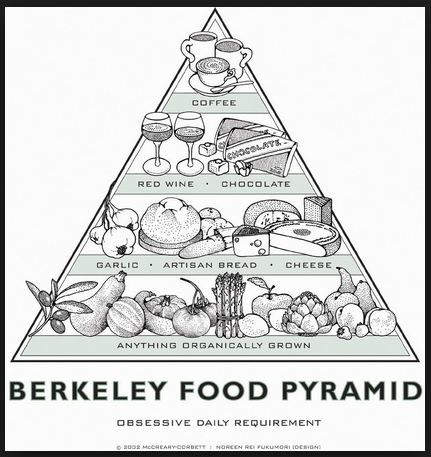
\includegraphics[width=0.5\linewidth,height=0.5\textheight]{pyramid} 

}

\caption{Berkeley Food Pyramid}\label{fig:pressure}
\end{figure}

\section{Introduction and
Explanation}\label{introduction-and-explanation}

In this report, we will examine the effects globalization in relation to
food on the climate. Taking inspiration from this cute image of the
``Berkeley Food Pyramid'', found in Peet's Coffee on 4th street, we will
examine what it means for cities worldwide to adopt foreign foods as
their own. In this example, we can see some products like wine, cheese,
and produce, especially garlic, are produced in California and not
shipped very far to come to Berkeley. However, other items like coffee
and chocolate have to be shipped from countries mainly in the global
south, like Colombia, Ethiopia, Vietnam, and Brazil.

Cheap, widely available oil makes it easier to ship all goods, including
food, all over the world, rather than engage in locally grown and
produced goods. Under longstanding trade agreements, fuel for
international freight carried by sea and air is not taxed. However, this
convenience comes at a cost to the environment. We are going to examine
the trends in US food imports, trends in carbon emissions in the US, as
well as global atmospheric CO2 concetrations during the same period.

While there are many contributing factors to climate change, the rise of
global CO2 emissions cannot be attributed solely to importing and
exporting food. This analysis will hopefully highlight the global
interconnectedness in all facets of trade and the way the current world
economy drives climate change.

The foods we studied were selected to mirror the ``Berkeley Food
Pyramid'' shown above, to depict this trend in a way that challenges the
idea that coffee and chocolate are part of Berkeley's food culture, and
to demonstrate that cities worldwide are accustomed to making certain
foods part of their culture without mind to the damage to the
environment that this practice causes.

\subsubsection{Information about the US Food Import Dataset, from the
data.gov
website}\label{information-about-the-us-food-import-dataset-from-the-data.gov-website}

\begin{quote}
U.S. consumers demand variety, quality, and convenience in the foods
they consume. As Americans have become wealthier and more ethnically
diverse, the American food basket reflects a growing share of tropical
products, spices, and imported gourmet products. Seasonal and climatic
factors drive U.S. imports of popular types of fruits and vegetables and
tropical products, such as cocoa and coffee. In addition, a growing
share of U.S. imports can be attributed to intra-industry trade, whereby
agricultural-processing industries based in the United States carry out
certain processing steps offshore and import products at different
levels of processing from their subsidiaries in foreign markets.
\end{quote}

This data set provides import values of edible products (food and
beverages) entering U.S. ports and their origin of shipment. Data are
from the U.S. Department of Commerce, U.S. Census Bureau. Food and
beverage import values are compiled by calendar year into food groups
corresponding to major commodities or level of processing. At least 10
years of annual data are included, enabling users to track long-term
growth patterns.

\emph{Volumes of food below is represented in units of 1000 metric
tons.}

\begin{Shaded}
\begin{Highlighting}[]
\NormalTok{berkeley_pyramid_imports <-}\StringTok{ }\KeywordTok{read_csv}\NormalTok{(}\StringTok{"Berkeley_Pyramid_Imports.csv"}\NormalTok{)}
\NormalTok{berkeley_pyramid_imports}
\end{Highlighting}
\end{Shaded}

\begin{verbatim}
## # A tibble: 7 x 20
##   X1    `1999` `2000` `2001` `2002` `2003` `2004` `2005` `2006` `2007`
##   <chr>  <dbl>  <dbl>  <dbl>  <dbl>  <dbl>  <dbl>  <dbl>  <dbl>  <dbl>
## 1 Coff~  3604.  3442.  2401.  2455.  2872.  3144.  3771.  4195.  4791.
## 2 Vege~  3632.  3771.  4157.  4391.  5082.  5730.  6043.  6619.  7256.
## 3 Fruit  4764.  4629.  4665.  5068.  5558.  5962.  6874.  7707.  9217.
## 4 Coco~  1522.  1404.  1536.  1761.  2439.  2484.  2751.  2659.  2662.
## 5 Chee~   705.   685.   746.   788.   882.   982.  1007.  1029.  1107.
## 6 Wine   2169.  2186.  2227.  2646.  3240.  3382.  3722.  4112.  4591.
## 7 Wheat   421.   382.   435.   463.   349.   443.   418.   581.   849.
## # ... with 10 more variables: `2008` <dbl>, `2009` <dbl>, `2010` <dbl>,
## #   `2011` <dbl>, `2012` <dbl>, `2013` <dbl>, `2014` <dbl>, `2015` <dbl>,
## #   `2016` <dbl>, `2017` <dbl>
\end{verbatim}

\begin{Shaded}
\begin{Highlighting}[]
\NormalTok{product_imports <-}\StringTok{ }\KeywordTok{read_csv}\NormalTok{(}\StringTok{"product_imports.csv"}\NormalTok{)}
\NormalTok{product_imports}
\end{Highlighting}
\end{Shaded}

\begin{verbatim}
## # A tibble: 133 x 3
##     Year Product              Quantity
##    <int> <chr>                   <dbl>
##  1  1999 Coffe & tea & spices    3604.
##  2  2000 Coffe & tea & spices    3442.
##  3  2001 Coffe & tea & spices    2401.
##  4  2002 Coffe & tea & spices    2455.
##  5  2003 Coffe & tea & spices    2872.
##  6  2004 Coffe & tea & spices    3144.
##  7  2005 Coffe & tea & spices    3771.
##  8  2006 Coffe & tea & spices    4195.
##  9  2007 Coffe & tea & spices    4791.
## 10  2008 Coffe & tea & spices    5581.
## # ... with 123 more rows
\end{verbatim}

\begin{Shaded}
\begin{Highlighting}[]
\NormalTok{cheese <-}\StringTok{ }\KeywordTok{filter}\NormalTok{(product_imports, Product }\OperatorTok{==}\StringTok{ "Cheese"}\NormalTok{)}
\NormalTok{vegetables <-}\StringTok{ }\KeywordTok{filter}\NormalTok{(product_imports, Product }\OperatorTok{==}\StringTok{ "Vegetables"}\NormalTok{)}
\NormalTok{wine <-}\StringTok{ }\KeywordTok{filter}\NormalTok{(product_imports, Product }\OperatorTok{==}\StringTok{ "Wine"}\NormalTok{)}
\NormalTok{fruit <-}\StringTok{ }\KeywordTok{filter}\NormalTok{(product_imports, Product }\OperatorTok{==}\StringTok{ "Fruit"}\NormalTok{)}
\NormalTok{cocoa <-}\StringTok{ }\KeywordTok{filter}\NormalTok{(product_imports, Product }\OperatorTok{==}\StringTok{ "Cocoa & chocolate"}\NormalTok{)}
\NormalTok{wheat <-}\StringTok{ }\KeywordTok{filter}\NormalTok{(product_imports, Product }\OperatorTok{==}\StringTok{ "Wheat"}\NormalTok{)}
\NormalTok{coffee <-}\StringTok{ }\KeywordTok{filter}\NormalTok{(product_imports, Product }\OperatorTok{==}\StringTok{ "Coffe & tea & spices"}\NormalTok{)}
\end{Highlighting}
\end{Shaded}

\begin{Shaded}
\begin{Highlighting}[]
\NormalTok{food_graph <-}\StringTok{ }
\StringTok{  }\KeywordTok{ggplot}\NormalTok{(, }\KeywordTok{aes}\NormalTok{(}\DataTypeTok{x =}\NormalTok{ Year)) }\OperatorTok{+}
\StringTok{  }\KeywordTok{geom_line}\NormalTok{(}\DataTypeTok{data =}\NormalTok{ cheese, }\KeywordTok{aes}\NormalTok{(}\DataTypeTok{y =}\NormalTok{ Quantity, }\DataTypeTok{color =} \StringTok{"cheese"}\NormalTok{)) }\OperatorTok{+}
\StringTok{  }\KeywordTok{geom_line}\NormalTok{(}\DataTypeTok{data =}\NormalTok{ wine, }\KeywordTok{aes}\NormalTok{(}\DataTypeTok{y =}\NormalTok{ Quantity, }\DataTypeTok{color =} \StringTok{"wine"}\NormalTok{)) }\OperatorTok{+}
\StringTok{  }\KeywordTok{geom_line}\NormalTok{(}\DataTypeTok{data =}\NormalTok{ vegetables, }\KeywordTok{aes}\NormalTok{(}\DataTypeTok{y =}\NormalTok{ Quantity, }\DataTypeTok{color =} \StringTok{"vegetables"}\NormalTok{)) }\OperatorTok{+}
\StringTok{  }\KeywordTok{geom_line}\NormalTok{(}\DataTypeTok{data =}\NormalTok{ fruit, }\KeywordTok{aes}\NormalTok{(}\DataTypeTok{y =}\NormalTok{ Quantity, }\DataTypeTok{color =} \StringTok{"fruit"}\NormalTok{)) }\OperatorTok{+}
\StringTok{  }\KeywordTok{geom_line}\NormalTok{(}\DataTypeTok{data =}\NormalTok{ coffee, }\KeywordTok{aes}\NormalTok{(}\DataTypeTok{y =}\NormalTok{ Quantity, }\DataTypeTok{color =} \StringTok{"coffee"}\NormalTok{)) }\OperatorTok{+}
\StringTok{  }\KeywordTok{geom_line}\NormalTok{(}\DataTypeTok{data =}\NormalTok{ cocoa, }\KeywordTok{aes}\NormalTok{(}\DataTypeTok{y =}\NormalTok{ Quantity, }\DataTypeTok{color =} \StringTok{"cocoa"}\NormalTok{)) }\OperatorTok{+}
\StringTok{  }\KeywordTok{geom_line}\NormalTok{(}\DataTypeTok{data =}\NormalTok{ wheat, }\KeywordTok{aes}\NormalTok{(}\DataTypeTok{y =}\NormalTok{ Quantity, }\DataTypeTok{color =} \StringTok{"wheat"}\NormalTok{)) }\OperatorTok{+}
\StringTok{  }\KeywordTok{scale_color_manual}\NormalTok{(}\StringTok{""}\NormalTok{,}
                     \DataTypeTok{breaks =} \KeywordTok{c}\NormalTok{(}\StringTok{"cheese"}\NormalTok{, }\StringTok{"wine"}\NormalTok{, }\StringTok{"vegetables"}\NormalTok{, }\StringTok{"fruit"}\NormalTok{, }\StringTok{"coffee"}\NormalTok{, }\StringTok{"cocoa"}\NormalTok{, }\StringTok{"wheat"}\NormalTok{),}
                     \DataTypeTok{values =} \KeywordTok{c}\NormalTok{(}\StringTok{"gold"}\NormalTok{, }\StringTok{"tan4"}\NormalTok{, }\StringTok{"black"}\NormalTok{, }\StringTok{"tomato"}\NormalTok{, }\StringTok{"forestgreen"}\NormalTok{, }\StringTok{"navajowhite"}\NormalTok{, }\StringTok{"maroon"}\NormalTok{)) }\OperatorTok{+}
\StringTok{  }\KeywordTok{theme_classic}\NormalTok{() }\OperatorTok{+}
\StringTok{  }\KeywordTok{labs}\NormalTok{(}\DataTypeTok{x =} \StringTok{"Year"}\NormalTok{, }\DataTypeTok{y =} \StringTok{"Quantity (1000 metric tons)"}\NormalTok{, }\DataTypeTok{title =} \StringTok{"Food Imports into the United States"}\NormalTok{)}
\NormalTok{food_graph}
\end{Highlighting}
\end{Shaded}

\includegraphics{Berkeley_Food_files/figure-latex/unnamed-chunk-11-1.pdf}

We can see in the graph above that the imports of fruit, vegetables, and
coffee saw the most dramatic increases in the last 15 years. All of
these food products are most commonly grown in the global south, meaning
that they must have traveled thousands of miles to reach Berkeley,
whether it be by land, sea, or air. Now if we assume that Berkeley saw a
fairly average decade during this period compared to the rest of the
country, it would make sense that the rest of the west coast - as well
as the rest of the United States - experienced a similar increase in
imports from the global south. Keep this in mind as we present the
carbon dioxide levels both globally and emitted by US transportation
below.

\subsubsection{Carbon Dioxide Emissions attributed to Transport in the
United
States}\label{carbon-dioxide-emissions-attributed-to-transport-in-the-united-states}

\emph{Data compiled from
\href{https://data.worldbank.org/indicator/EN.CO2.TRAN.ZS?end=2014\&locations=US\&start=1999}{The
World Bank} online database.}

\begin{Shaded}
\begin{Highlighting}[]
\NormalTok{test <-}\StringTok{ }\KeywordTok{GET}\NormalTok{(}\StringTok{"http://api.worldbank.org/v2/en/indicator/EN.CO2.TRAN.ZS?downloadformat=csv"}\NormalTok{, }
            \KeywordTok{write_disk}\NormalTok{(}\StringTok{"test.zip"}\NormalTok{, }\DataTypeTok{overwrite =} \OtherTok{TRUE}\NormalTok{))}
  \KeywordTok{unzip}\NormalTok{(}\StringTok{"test.zip"}\NormalTok{)}

\NormalTok{co2_info <-}\StringTok{ }\KeywordTok{read_csv}\NormalTok{(}\StringTok{"API_EN.CO2.TRAN.ZS_DS2_en_csv_v2_10228633.csv"}\NormalTok{,}
                     \DataTypeTok{skip =} \DecValTok{4}\NormalTok{)}

\NormalTok{unitedstates_co2 <-}\StringTok{ }\NormalTok{co2_info }\OperatorTok
\StringTok{  }\KeywordTok{select}\NormalTok{(}\StringTok{"Country Name"}\NormalTok{, }\StringTok{"1999"}\OperatorTok{:}\StringTok{"2014"}\NormalTok{) }\OperatorTok
\StringTok{  }\KeywordTok{slice}\NormalTok{(}\DecValTok{250}\NormalTok{)}
\NormalTok{unitedstates_co2}
\end{Highlighting}
\end{Shaded}

\begin{verbatim}
## # A tibble: 1 x 17
##   `Country Name` `1999` `2000` `2001` `2002` `2003` `2004` `2005` `2006`
##   <chr>           <dbl>  <dbl>  <dbl>  <dbl>  <dbl>  <dbl>  <dbl>  <dbl>
## 1 United States    31.0   30.4   30.7   31.5   31.5   31.4   31.7   32.2
## # ... with 8 more variables: `2007` <dbl>, `2008` <dbl>, `2009` <dbl>,
## #   `2010` <dbl>, `2011` <dbl>, `2012` <dbl>, `2013` <dbl>, `2014` <dbl>
\end{verbatim}

\begin{Shaded}
\begin{Highlighting}[]
\NormalTok{table <-}\StringTok{ }\NormalTok{unitedstates_co2 }\OperatorTok
\StringTok{  }\KeywordTok{gather}\NormalTok{(}\StringTok{"Country Name"}\NormalTok{, }\StringTok{"Year"}\NormalTok{)}

\KeywordTok{names}\NormalTok{(table)[}\DecValTok{1}\NormalTok{] <-}\StringTok{ "Date"}
\KeywordTok{names}\NormalTok{(table)[}\DecValTok{2}\NormalTok{] <-}\StringTok{ "Co2"}

\NormalTok{table}
\end{Highlighting}
\end{Shaded}

\begin{verbatim}
## # A tibble: 16 x 2
##    Date    Co2
##    <chr> <dbl>
##  1 1999   31.0
##  2 2000   30.4
##  3 2001   30.7
##  4 2002   31.5
##  5 2003   31.5
##  6 2004   31.4
##  7 2005   31.7
##  8 2006   32.2
##  9 2007   31.8
## 10 2008   31.0
## 11 2009   31.7
## 12 2010   31.3
## 13 2011   31.7
## 14 2012   33.6
## 15 2013   33.1
## 16 2014   33.4
\end{verbatim}

\begin{Shaded}
\begin{Highlighting}[]
\NormalTok{usplot <-}\StringTok{ }\KeywordTok{ggplot}\NormalTok{(table, }\KeywordTok{aes}\NormalTok{(}\DataTypeTok{x =}\NormalTok{ Date, }\DataTypeTok{y =}\NormalTok{ Co2, }\DataTypeTok{group =} \DecValTok{1}\NormalTok{)) }\OperatorTok{+}\StringTok{ }\KeywordTok{geom_smooth}\NormalTok{() }\OperatorTok{+}\StringTok{ }
\StringTok{  }\KeywordTok{ggtitle}\NormalTok{(}\StringTok{"CO2 Emissions from Transport in United States"}\NormalTok{) }\OperatorTok{+}\StringTok{ }
\StringTok{  }\KeywordTok{ylab}\NormalTok{(}\StringTok{"% of CO2 Emissions from Transport"}\NormalTok{) }\OperatorTok{+}
\StringTok{  }\KeywordTok{xlab}\NormalTok{(}\StringTok{"Year"}\NormalTok{)}
\NormalTok{usplot}
\end{Highlighting}
\end{Shaded}

\includegraphics{Berkeley_Food_files/figure-latex/unnamed-chunk-12-1.pdf}

According to this graphic, the percentage of carbon dioxide emissions
contributed by transportation rose from around 30.5\% to almost 34\% in
the same time period as we saw the increase in imports. This data along
with the following global atmospheric carbon dioxide data should paint a
correlative picture of rising emissions and climate change.

\subsubsection{Atmospheric Carbon Dioxide
Data}\label{atmospheric-carbon-dioxide-data}

\emph{Data sourced from
\href{https://climate.nasa.gov/vital-signs/carbon-dioxide/}{NASA}}

\begin{Shaded}
\begin{Highlighting}[]
\NormalTok{co2 <-}
\NormalTok{readr}\OperatorTok{::}\KeywordTok{read_table}\NormalTok{(}\StringTok{"ftp://aftp.cmdl.noaa.gov/products/trends/co2/co2_mm_mlo.txt"}\NormalTok{,}
                  \DataTypeTok{comment =} \StringTok{"#"}\NormalTok{,}
                  \DataTypeTok{col_names =} \KeywordTok{c}\NormalTok{(}\StringTok{"year"}\NormalTok{, }\StringTok{"month"}\NormalTok{, }\StringTok{"decimal_date"}\NormalTok{, }\StringTok{"average"}\NormalTok{,}
                                \StringTok{"interpolated"}\NormalTok{, }\StringTok{"trend"}\NormalTok{, }\StringTok{"days"}\NormalTok{),}
                  \DataTypeTok{na =} \KeywordTok{c}\NormalTok{(}\StringTok{"-1"}\NormalTok{, }\StringTok{"-99.99"}\NormalTok{))}
\end{Highlighting}
\end{Shaded}

\begin{Shaded}
\begin{Highlighting}[]
\NormalTok{berkeley_co2 <-}\StringTok{ }\KeywordTok{filter}\NormalTok{(co2, year }\OperatorTok{>=}\StringTok{ "1999"}\NormalTok{, year }\OperatorTok{<=}\StringTok{ "2017"}\NormalTok{)}
\NormalTok{berkeley_co2}
\end{Highlighting}
\end{Shaded}

\begin{verbatim}
## # A tibble: 228 x 7
##     year month decimal_date average interpolated trend  days
##    <int> <int>        <dbl>   <dbl>        <dbl> <dbl> <int>
##  1  1999     1        1999.    368.         368.  368.    27
##  2  1999     2        1999.    369.         369.  368.    22
##  3  1999     3        1999.    370.         370.  368.    25
##  4  1999     4        1999.    371.         371.  368.    29
##  5  1999     5        1999.    371.         371.  368.    26
##  6  1999     6        1999.    370.         370.  368.    26
##  7  1999     7        2000.    369.         369.  369.    27
##  8  1999     8        2000.    367.         367.  368.    25
##  9  1999     9        2000.    365.         365.  368.    28
## 10  1999    10        2000.    365.         365.  369.    31
## # ... with 218 more rows
\end{verbatim}

\begin{Shaded}
\begin{Highlighting}[]
\NormalTok{co2_plot <-}
\KeywordTok{ggplot}\NormalTok{(berkeley_co2, }\KeywordTok{aes}\NormalTok{(}\DataTypeTok{x =}\NormalTok{ year, }\DataTypeTok{y =}\NormalTok{ average)) }\OperatorTok{+}\StringTok{ }\KeywordTok{geom_smooth}\NormalTok{() }\OperatorTok{+}
\StringTok{  }\KeywordTok{labs}\NormalTok{( }\DataTypeTok{x =} \StringTok{"Year"}\NormalTok{, }\DataTypeTok{y =} \StringTok{"Average Annual CO2 (ppm)"}\NormalTok{, }\DataTypeTok{title =} \StringTok{"Global CO2 Concentration: 1999-2017"}\NormalTok{) }\OperatorTok{+}\StringTok{ }\KeywordTok{ylim}\NormalTok{(}\DecValTok{300}\NormalTok{, }\DecValTok{450}\NormalTok{) }
\NormalTok{co2_plot}
\end{Highlighting}
\end{Shaded}

\includegraphics{Berkeley_Food_files/figure-latex/unnamed-chunk-15-1.pdf}

\subsubsection{Conclusion}\label{conclusion}

In conclusion, while we cannot draw any conclusions that the global food
market is driving climate change, we believe that there is enough
evidence (as presented above) to suggest that it is in fact a
contributing factor. To combat this increase, one suggestion is to move
towards a more localized diet. This would support local farmers and also
has been shown to influence communities towards a healthier, fresher,
more sustainable diet.


\end{document}
